\documentclass[12pt,twoside]{article}
\usepackage{chadstyle}  % Loads my formatting 
\usepackage{pgffor}
\usepackage{tikz}
\usepackage{subcaption}
\usepackage{longtable}
\usepackage{color, colortbl}
\usepackage{booktabs}
\usepackage{pgfplots}
\usepackage{bm}
\usepackage{hyperref}
%\usepackage{minipage}
%\usetikzlibrary{positioning}
\usepgfplotslibrary{groupplots}
\numberwithin{equation}{section}
%\usepackage[demo]{graphicx} % "demo" option just for this example
\usepackage{floatrow}
\DeclareFloatVCode{somespace}{\vspace{1.667\baselineskip}}
\floatsetup{rowpostcode =somespace, margins = centering}
\newtheorem{example}{Example}
\definecolor{red}{rgb}{0.549019608,0.082352941,0.082352941} %{.5,0,.5}
\definecolor{blue}{rgb}{.1,.1,.5}  
\definecolor{green}{rgb}{0,.4,0}    % Dark Green
\begin{document}
\bibliographystyle{aernobold}

%%%%%%%%%%%%%%%%%%%%%%%%%%%%%%%%%%%%%%%%%%%%%%%%%%%%%%%%%%%%%%%%%
% TITLE PAGE
%%%%%%%%%%%%%%%%%%%%%%%%%%%%%%%%%%%%%%%%%%%%%%%%%%%%%%%%%%%%%%%%%

%\begin{singlespacing}
%\begin{spacing}{0.9}
%\begin{titlepage}

%Two authors: \author{Matthias Doepke\\{\small UCLA, NBER, CEPR, and IZA}
%\and Mich\`{e}le Tertilt\\
%{\small Stanford University, NBER, and CEPR}}

\title{Section \# 1 -- ECON 102A}
\runningheads{Daniele Caratelli}{Section \#1 -- ECON 102A}


\author{\large Daniele Caratelli\\ {Stanford University}
%{\normalsize \url{http://www.econ.berkeley.edu/~chad}}
}
%, for his guidance and feedback which brought me back on course whenever my thoughts led me astray. 

\date{\small \today }
\maketitle
\thispagestyle{empty}

%\clearpage
\vspace{-0.3in}

\tableofcontents

\clearpage

\section{Making sure we get the definitions}

\begin{enumerate}
	\item[] %\textbf{Sample space:} is the collection of all possible outcomes.\\	
	\begin{example}
	Suppose there is a game where, if you toss a die and get either a 1 or a 6 you win \$100, otherwise you get nothing. What is the \textcolor{ChadRed}{sample space}?
		\begin{enumerate}
			\item $S=\$100$
			\item $S=\{1,6\}$
			\item $S=\{1,2,3,4,5,6\}$
			\item $S=\{1,2,3,4,5,6,7\}$
		\end{enumerate}
	\end{example}
	
	\item[] %\textbf{Event:} is one or a collection of possible outcomes.
	\begin{example}
		I roll 2 dice and record the face value of the first and second toss (\#1, \#2). Which of these is an \textcolor{red}{outcome}, which is an \textcolor{red}{event}, and which is the \textcolor{red}{sample space}?
		\begin{enumerate}
			\item $(6,2)$
			\item $\left\{(6,2), (5,2)\right\}$
			\item $\left\{(1,1), (1,2), (1,3), (1,4), (1,5), (1,6), (2,1) \dots, (6,4), (6,5), (6,6)\right\}$
		\end{enumerate}
	\end{example}


\end{enumerate}

\clearpage
\section{Trees and Bayes' rule}
\subsection{Constructing a probability tree}
A tree is an easy way to visualize probabilistic outcomes. I show a simple recipe to write down probability trees - though they are easier done than said!
\begin{enumerate}
	\item Draw an initial node. Nothing has happened yet - you cannot go wrong at the initial node!\vspace*{-1em}
	\item From each node, draw branches: branches indicate something is uncertain, multiple events could be realized. At any given node there will as many branches as there are possible outcomes at that stage.\vspace*{-1em}
	\item On top of the branches it is useful to write the probability of that outcome occurring.\vspace*{-1em}
	\item Trees can have different stages. Stages can indicate different events (e.g. problem may ask to consider event A and B, stage 1 would deal with the first event, stage 2 with the second). It can also display different period of the game (e.g. 1st, 2nd, 3rd draw).
\end{enumerate}

\noindent $\bm{\longrightarrow}$ very useful to study operations and in general whenever we apply operations on event


\begin{figure}[htpb!]
	\centering

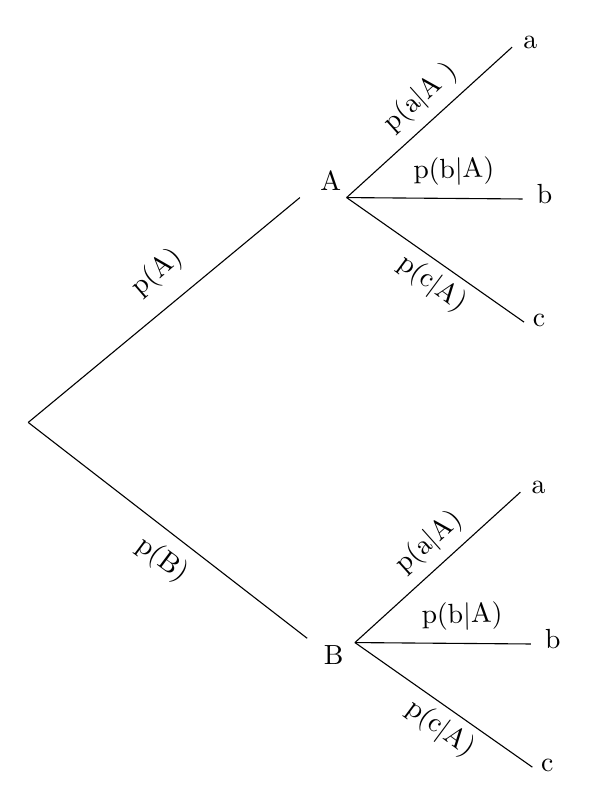
\begin{tikzpicture}[x=0.75pt,y=0.75pt,yscale=-1,xscale=1,scale=1.2]
\draw    (70,322.1) -- (182,408.77) ;
\draw    (70,322.1) -- (179.07,231.82) ;
\draw    (197.83,231.82) -- (268.47,232.38) ;
\draw    (264.27,171.42) -- (197.83,231.82) ;
\draw    (197.83,231.82) -- (269.07,281.82) ;
\draw    (201.17,410.48) -- (271.8,411.05) ;
\draw    (267.6,350.09) -- (201.17,410.48) ;
\draw    (201.17,410.48) -- (272.4,460.49) ;


\draw (191.47,225.3) node   [align=left] {A};
\draw (271.47,169.7) node   [align=left] {a};
\draw (277.27,230.4) node   [align=left] {b};
\draw (275.07,281.1) node   [align=left] {c};
\draw (192.67,415.5) node   [align=left] {B};
\draw (121.67,262) node  [rotate=-319.14] [align=left] {p(A)};
\draw (123.67,377.33) node  [rotate=-36.71] [align=left] {p(B)};
\draw (227.47,191.6) node  [rotate=-318.24] [align=left] {p(a$\vert$A )};
\draw (240.87,221.2) node  [rotate=-359.14] [align=left] {p(b$\vert$A)};
\draw (232.07,266.4) node  [rotate=-36.54] [align=left] {p(c$\vert$A)};
\draw (274.8,348.37) node   [align=left] {a};
\draw (280.6,409.07) node   [align=left] {b};
\draw (278.4,459.77) node   [align=left] {c};
\draw (230.8,370.27) node  [rotate=-318.24] [align=left] {p(a$\vert$A)};
\draw (244.2,399.87) node  [rotate=-359.14] [align=left] {p(b$\vert$A)};
\draw (235.4,445.07) node  [rotate=-36.54] [align=left] {p(c$\vert$A)};
\end{tikzpicture}
\caption{Sample probability tree}
\end{figure}\clearpage


\subsection{Operations on trees}

Trees are very useful anytime you do \textcolor{red}{operations on probabilities}.

\begin{enumerate}
	\item[] \textbf{\textcolor{red}{Intersection:}}\\
	$P(A \cap a) = P(Aa)$ is the probability that both $A$ and $a$ occur (see Figure \ref{fig:intersection}). Recall: $$P(A \cap a) = P(Aa) = P(a|A)\cdot P(A).$$
	\begin{figure}[htpb!]
		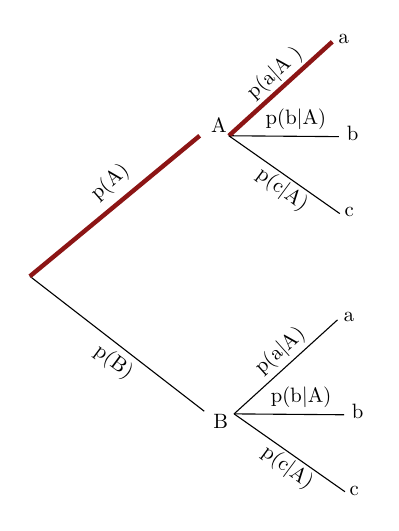
\begin{tikzpicture}[x=0.75pt,y=0.75pt,yscale=-1,xscale=1,scale=0.75,every node/.style={scale=0.75}]
		\draw    (70,322.1) -- (182,408.77) ;
		\draw[ultra thick,red]    (70,322.1) -- (179.07,231.82) ;
		\draw    (197.83,231.82) -- (268.47,232.38) ;
		\draw[ultra thick,red]    (197.83,231.82) -- (264.27,171.42) ;
		\draw    (197.83,231.82) -- (269.07,281.82) ;
		\draw    (201.17,410.48) -- (271.8,411.05) ;
		\draw    (267.6,350.09) -- (201.17,410.48) ;
		\draw    (201.17,410.48) -- (272.4,460.49) ;
		
		
		\draw (191.47,225.3) node   [align=left] {A};
		\draw (271.47,169.7) node   [align=left] {a};
		\draw (277.27,230.4) node   [align=left] {b};
		\draw (275.07,281.1) node   [align=left] {c};
		\draw (192.67,415.5) node   [align=left] {B};
		\draw (121.67,262) node  [rotate=-319.14] [align=left] {p(A)};
		\draw (123.67,377.33) node  [rotate=-36.71] [align=left] {p(B)};
		\draw (227.47,191.6) node  [rotate=-318.24] [align=left] {p(a$\vert$A )};
		\draw (240.87,221.2) node  [rotate=-359.14] [align=left] {p(b$\vert$A)};
		\draw (232.07,266.4) node  [rotate=-36.54] [align=left] {p(c$\vert$A)};
		\draw (274.8,348.37) node   [align=left] {a};
		\draw (280.6,409.07) node   [align=left] {b};
		\draw (278.4,459.77) node   [align=left] {c};
		\draw (230.8,370.27) node  [rotate=-318.24] [align=left] {p(a$\vert$A)};
		\draw (244.2,399.87) node  [rotate=-359.14] [align=left] {p(b$\vert$A)};
		\draw (235.4,445.07) node  [rotate=-36.54] [align=left] {p(c$\vert$A)};
		\end{tikzpicture}
		\caption{Intersection}
		\label{fig:intersection}
	\end{figure}
	
	\item[] \textbf{\textcolor{red}{Union:}}\\
	$P(A\cup a)$ is the probability that \textit{either} $A$ or $a$ occurred (see Figure \ref{fig:union}). Recall:
	$$P(A \cap a) = \textcolor{red}{\bm{P(A)}}+\textcolor{blue}{\bm{P(a)}}-\textcolor{green}{\bm{P(Aa)}}.$$

	\begin{figure}[htpb!]
		\centering
		\begin{subfigure}{0.35\textwidth}
			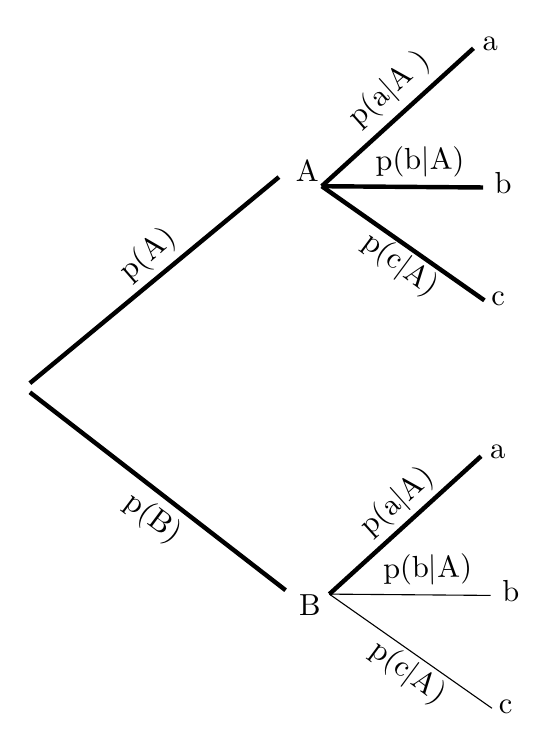
\begin{tikzpicture}[x=0.75pt,y=0.75pt,yscale=-1,xscale=1,scale=1.1,every node/.style={scale=1.1}]
			\draw[ultra thick,black]    (70,322.1) -- (182,408.77) ;
			\draw[ultra thick,black]    (70,318.1) -- (179.07,227.82) ;
			\draw[ultra thick,black]    (197.83,231.82) -- (268.47,232.38) ;
			\draw[ultra thick,black] (264.27,171.42) -- (197.83,231.82) ;
			\draw[ultra thick,black]    (197.83,231.82) -- (269.07,281.82) ;
			\draw    (201.17,410.48) -- (271.8,411.05) ;
			\draw[ultra thick,black]    (267.6,350.09) -- (201.17,410.48) ;
			\draw    (201.17,410.48) -- (272.4,460.49) ;
			
			
			\draw (191.47,225.3) node   [align=left] {A};
			\draw (271.47,169.7) node   [align=left] {a};
			\draw (277.27,230.4) node   [align=left] {b};
			\draw (275.07,281.1) node   [align=left] {c};
			\draw (192.67,415.5) node   [align=left] {B};
			\draw (121.67,262) node  [rotate=-319.14] [align=left] {p(A)};
			\draw (123.67,377.33) node  [rotate=-36.71] [align=left] {p(B)};
			\draw (227.47,189.6) node  [rotate=-318.24] [align=left] {p(a$\vert$A )};
			\draw (240.87,221.2) node  [rotate=-359.14] [align=left] {p(b$\vert$A)};
			\draw (232.07,266.4) node  [rotate=-36.54] [align=left] {p(c$\vert$A)};
			\draw (274.8,348.37) node   [align=left] {a};
			\draw (280.6,409.07) node   [align=left] {b};
			\draw (278.4,459.77) node   [align=left] {c};
			\draw (230.8,370.27) node  [rotate=-318.24] [align=left] {p(a$\vert$A)};
			\draw (244.2,399.87) node  [rotate=-359.14] [align=left] {p(b$\vert$A)};
			\draw (235.4,445.07) node  [rotate=-36.54] [align=left] {p(c$\vert$A)};
			\end{tikzpicture}
		\end{subfigure}
		\hspace*{\fill}
		\begin{subfigure}{0.55\textwidth}
			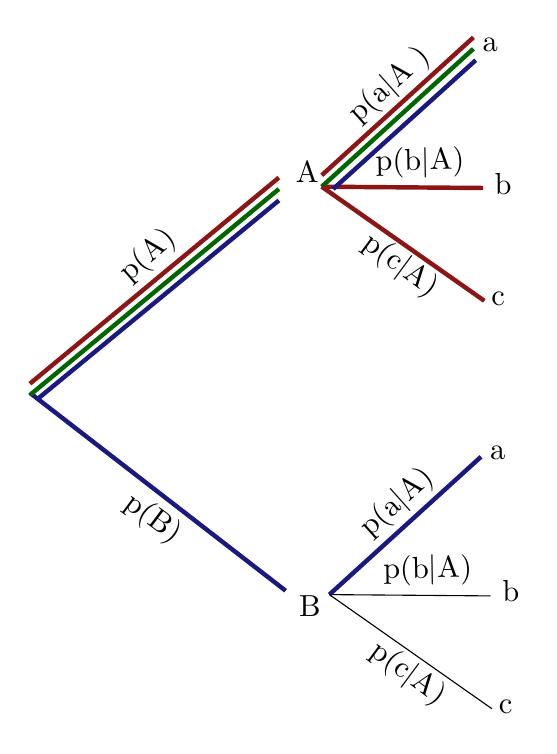
\begin{tikzpicture}[x=0.75pt,y=0.75pt,yscale=-1,xscale=1,scale=1.1,every node/.style={scale=1.1}]
			\draw[ultra thick,blue]    (70,322.1) -- (182,408.77) ;
			\draw[ultra thick,red]    (70,318.1) -- (179.07,227.82) ;
			\draw[ultra thick,green]    (70,323.1) -- (179.07,232.82) ;
			\draw[ultra thick,blue]    (73,325.1) -- (179.07,237.82) ;
			\draw[ultra thick,red]    (197.83,231.82) -- (268.47,232.38) ;
			\draw[ultra thick,red]    (264.27,166.42) -- (197.83,226.82) ;
			\draw[ultra thick,green] (264.27,171.42) -- (197.83,231.82) ;
			\draw[ultra thick,blue] (202.83,232.82) -- (265.27,176.42) ;
			\draw[ultra thick,red]    (197.83,231.82) -- (269.07,281.82) ;
			\draw    (201.17,410.48) -- (271.8,411.05) ;
			\draw[ultra thick,blue]    (267.6,350.09) -- (201.17,410.48) ;
			\draw    (201.17,410.48) -- (272.4,460.49) ;
			
			
			\draw (191.47,225.3) node   [align=left] {A};
			\draw (271.47,169.7) node   [align=left] {a};
			\draw (277.27,230.4) node   [align=left] {b};
			\draw (275.07,281.1) node   [align=left] {c};
			\draw (192.67,415.5) node   [align=left] {B};
			\draw (121.67,262) node  [rotate=-319.14] [align=left] {p(A)};
			\draw (123.67,377.33) node  [rotate=-36.71] [align=left] {p(B)};
			\draw (227.47,187.6) node  [rotate=-318.24] [align=left] {p(a$\vert$A )};
			\draw (240.87,221.2) node  [rotate=-359.14] [align=left] {p(b$\vert$A)};
			\draw (232.07,266.4) node  [rotate=-36.54] [align=left] {p(c$\vert$A)};
			\draw (274.8,348.37) node   [align=left] {a};
			\draw (280.6,409.07) node   [align=left] {b};
			\draw (278.4,459.77) node   [align=left] {c};
			\draw (230.8,370.27) node  [rotate=-318.24] [align=left] {p(a$\vert$A)};
			\draw (244.2,399.87) node  [rotate=-359.14] [align=left] {p(b$\vert$A)};
			\draw (235.4,445.07) node  [rotate=-36.54] [align=left] {p(c$\vert$A)};
			\end{tikzpicture}
		\end{subfigure}
		\caption{Union}
		\label{fig:union}
	\end{figure}
	
	\item[] \textbf{\textcolor{red}{Conditional:}}\\
	$P(a|A)$ is the probability that $a$ occurred given $A$ has occurred, in other words we already know some information about what has happened (see Figure \ref{fig:conditional}). Recall:
	$$P(a|A) = \frac{P(A\cap a)}{P(A)} = \frac{P(Aa)}{P(A)} = \frac{\textcolor{red}{\bm{P(Aa)}}}{\textcolor{blue}{\bm{P(A)}}}.$$
	
	\begin{figure}[htpb!]
		\centering
		\begin{subfigure}{0.45\textwidth}
			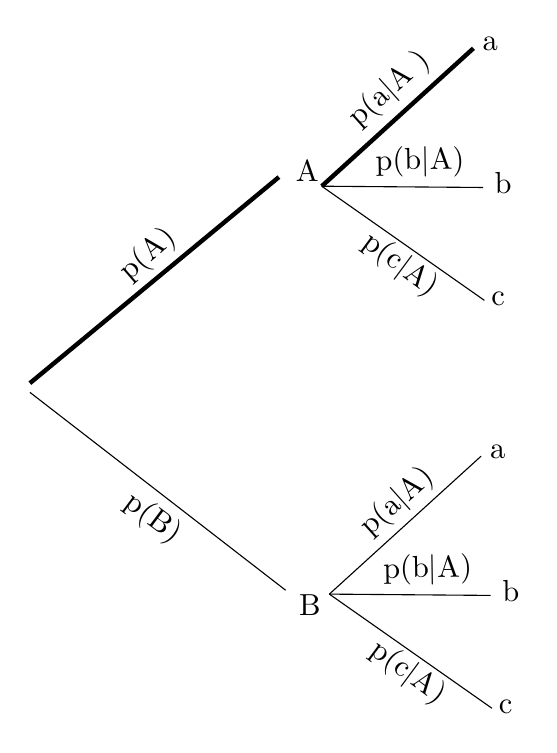
\begin{tikzpicture}[x=0.75pt,y=0.75pt,yscale=-1,xscale=1,scale=1.1,every node/.style={scale=1.1}]
			\draw    (70,322.1) -- (182,408.77) ;
			\draw[ultra thick,black]    (70,318.1) -- (179.07,227.82) ;
			\draw    (197.83,231.82) -- (268.47,232.38) ;
			\draw[ultra thick,black] (264.27,171.42) -- (197.83,231.82) ;
			\draw    (197.83,231.82) -- (269.07,281.82) ;
			\draw    (201.17,410.48) -- (271.8,411.05) ;
			\draw    (267.6,350.09) -- (201.17,410.48) ;
			\draw    (201.17,410.48) -- (272.4,460.49) ;
			
			
			\draw (191.47,225.3) node   [align=left] {A};
			\draw (271.47,169.7) node   [align=left] {a};
			\draw (277.27,230.4) node   [align=left] {b};
			\draw (275.07,281.1) node   [align=left] {c};
			\draw (192.67,415.5) node   [align=left] {B};
			\draw (121.67,262) node  [rotate=-319.14] [align=left] {p(A)};
			\draw (123.67,377.33) node  [rotate=-36.71] [align=left] {p(B)};
			\draw (227.47,189.6) node  [rotate=-318.24] [align=left] {p(a$\vert$A )};
			\draw (240.87,221.2) node  [rotate=-359.14] [align=left] {p(b$\vert$A)};
			\draw (232.07,266.4) node  [rotate=-36.54] [align=left] {p(c$\vert$A)};
			\draw (274.8,348.37) node   [align=left] {a};
			\draw (280.6,409.07) node   [align=left] {b};
			\draw (278.4,459.77) node   [align=left] {c};
			\draw (230.8,370.27) node  [rotate=-318.24] [align=left] {p(a$\vert$A)};
			\draw (244.2,399.87) node  [rotate=-359.14] [align=left] {p(b$\vert$A)};
			\draw (235.4,445.07) node  [rotate=-36.54] [align=left] {p(c$\vert$A)};
			\end{tikzpicture}
		\end{subfigure}
		\hspace*{\fill}
		\begin{subfigure}{0.45\textwidth}
			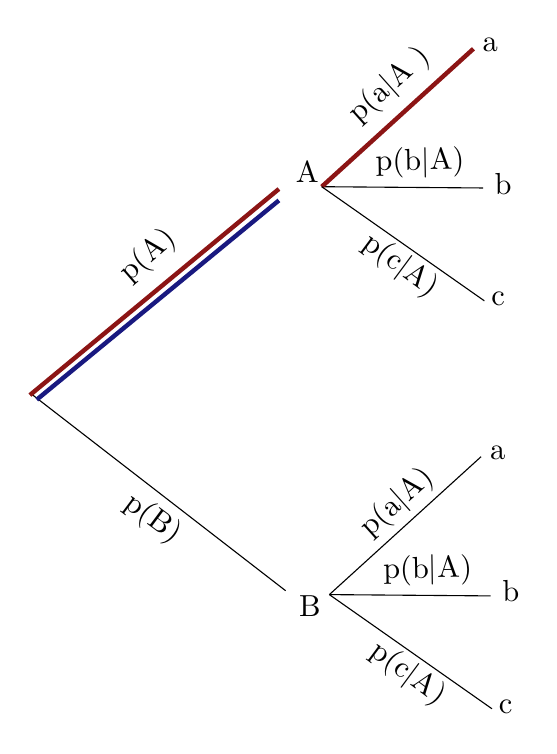
\begin{tikzpicture}[x=0.75pt,y=0.75pt,yscale=-1,xscale=1,scale=1.1,every node/.style={scale=1.1}]
			\draw    (70,322.1) -- (182,408.77) ;
			\draw[ultra thick,red]    (70,323.1) -- (179.07,232.82) ;
			\draw[ultra thick,blue]    (73,325.1) -- (179.07,237.82) ;
			\draw    (197.83,231.82) -- (268.47,232.38) ;
			\draw[ultra thick,red] (264.27,171.42) -- (197.83,231.82) ;
			\draw    (197.83,231.82) -- (269.07,281.82) ;
			\draw    (201.17,410.48) -- (271.8,411.05) ;
			\draw    (267.6,350.09) -- (201.17,410.48) ;
			\draw    (201.17,410.48) -- (272.4,460.49) ;
			
			
			\draw (191.47,225.3) node   [align=left] {A};
			\draw (271.47,169.7) node   [align=left] {a};
			\draw (277.27,230.4) node   [align=left] {b};
			\draw (275.07,281.1) node   [align=left] {c};
			\draw (192.67,415.5) node   [align=left] {B};
			\draw (121.67,262) node  [rotate=-319.14] [align=left] {p(A)};
			\draw (123.67,377.33) node  [rotate=-36.71] [align=left] {p(B)};
			\draw (227.47,187.6) node  [rotate=-318.24] [align=left] {p(a$\vert$A )};
			\draw (240.87,221.2) node  [rotate=-359.14] [align=left] {p(b$\vert$A)};
			\draw (232.07,266.4) node  [rotate=-36.54] [align=left] {p(c$\vert$A)};
			\draw (274.8,348.37) node   [align=left] {a};
			\draw (280.6,409.07) node   [align=left] {b};
			\draw (278.4,459.77) node   [align=left] {c};
			\draw (230.8,370.27) node  [rotate=-318.24] [align=left] {p(a$\vert$A)};
			\draw (244.2,399.87) node  [rotate=-359.14] [align=left] {p(b$\vert$A)};
			\draw (235.4,445.07) node  [rotate=-36.54] [align=left] {p(c$\vert$A)};
			\end{tikzpicture}
		\end{subfigure}
		\caption{Conditional}
		\label{fig:conditional}
	\end{figure}
	
	
	\subsection{Flipping trees}
	Suppose there are events $A$ and $B$, the original tree has $A$ first and $B$ second.
	\begin{enumerate}
		\item \textbf{Step 1:} Switch order of events and allocate terminal probabilities accordingly (this just means rearrange so that the probabilities are in the right place and consistent with the un-flipped tree).
		\item \textbf{Step 2:} Determine the \textit{new} initial probabilities, i.e. go from conditional to unconditional probabilities ($P(B|A)\rightarrow P(B)$).
		\item \textbf{Step 3:} Determine the \textit{new} conditional probabilities by dividing the terminal probabilities by the appropriate initial probabilities.
	\end{enumerate}
\end{enumerate}


	\subsection{Venn Diagrams}
	Venn diagrams can be helpful to visualize probabilities. Sometimes also to compute some operations with probabilities (union and intersection). I think that Venn diagrams are particularly useful when going from raw numbers to probabilities, or when showing mathematical relationships actually hold.\\	
	It is important to construct the diagram so the intersections, unions, and the like are correct. Which is ``more" correct in Figure \ref{fig:venn}?
	

	
	\begin{figure}[htpb!]
		\centering 
		\tikzset{every picture/.style={line width=0.75pt}} %set default line width to 0.75pt        
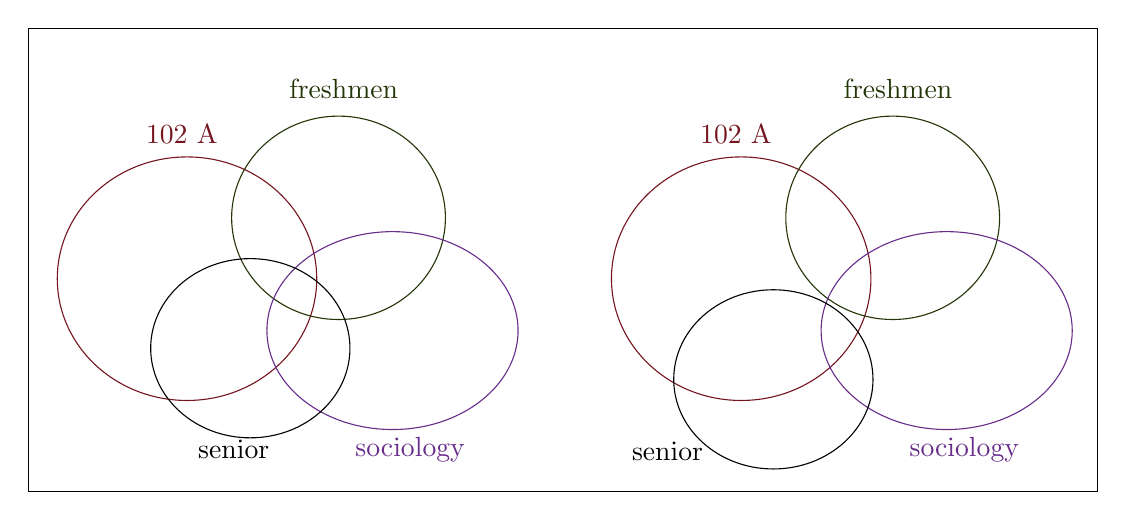
\begin{tikzpicture}[x=0.75pt,y=0.75pt,yscale=-1,xscale=1]
%uncomment if require: \path (0,553); %set diagram left start at 0, and has height of 553

%Shape: Rectangle [id:dp0440252950188863] 
\draw   (62,221.33) -- (577,221.33) -- (577,444.67) -- (62,444.67) -- cycle ;
%Flowchart: Connector [id:dp7859945077609718] 
\draw  [color={rgb, 255:red, 208; green, 2; blue, 27 }  ,draw opacity=1 ] (76,342) .. controls (76,309.6) and (103.98,283.33) .. (138.5,283.33) .. controls (173.02,283.33) and (201,309.6) .. (201,342) .. controls (201,374.4) and (173.02,400.67) .. (138.5,400.67) .. controls (103.98,400.67) and (76,374.4) .. (76,342) -- cycle ;
%Flowchart: Connector [id:dp002543642332927365] 
\draw  [color={rgb, 255:red, 65; green, 117; blue, 5 }  ,draw opacity=1 ] (160,312.67) .. controls (160,285.6) and (183.06,263.67) .. (211.5,263.67) .. controls (239.94,263.67) and (263,285.6) .. (263,312.67) .. controls (263,339.73) and (239.94,361.67) .. (211.5,361.67) .. controls (183.06,361.67) and (160,339.73) .. (160,312.67) -- cycle ;
%Flowchart: Connector [id:dp48556643719259573] 
\draw  [color={rgb, 255:red, 144; green, 19; blue, 254 }  ,draw opacity=1 ] (177,367) .. controls (177,340.67) and (204.09,319.33) .. (237.5,319.33) .. controls (270.91,319.33) and (298,340.67) .. (298,367) .. controls (298,393.33) and (270.91,414.67) .. (237.5,414.67) .. controls (204.09,414.67) and (177,393.33) .. (177,367) -- cycle ;
%Flowchart: Connector [id:dp2587248955701891] 
\draw   (121,375.5) .. controls (121,351.66) and (142.49,332.33) .. (169,332.33) .. controls (195.51,332.33) and (217,351.66) .. (217,375.5) .. controls (217,399.34) and (195.51,418.67) .. (169,418.67) .. controls (142.49,418.67) and (121,399.34) .. (121,375.5) -- cycle ;
%Flowchart: Connector [id:dp9308575791082676] 
\draw  [color={rgb, 255:red, 208; green, 2; blue, 27 }  ,draw opacity=1 ] (343,342) .. controls (343,309.6) and (370.98,283.33) .. (405.5,283.33) .. controls (440.02,283.33) and (468,309.6) .. (468,342) .. controls (468,374.4) and (440.02,400.67) .. (405.5,400.67) .. controls (370.98,400.67) and (343,374.4) .. (343,342) -- cycle ;
%Flowchart: Connector [id:dp32438083016663055] 
\draw  [color={rgb, 255:red, 65; green, 117; blue, 5 }  ,draw opacity=1 ] (427,312.67) .. controls (427,285.6) and (450.06,263.67) .. (478.5,263.67) .. controls (506.94,263.67) and (530,285.6) .. (530,312.67) .. controls (530,339.73) and (506.94,361.67) .. (478.5,361.67) .. controls (450.06,361.67) and (427,339.73) .. (427,312.67) -- cycle ;
%Flowchart: Connector [id:dp8092302400304977] 
\draw  [color={rgb, 255:red, 144; green, 19; blue, 254 }  ,draw opacity=1 ] (444,367) .. controls (444,340.67) and (471.09,319.33) .. (504.5,319.33) .. controls (537.91,319.33) and (565,340.67) .. (565,367) .. controls (565,393.33) and (537.91,414.67) .. (504.5,414.67) .. controls (471.09,414.67) and (444,393.33) .. (444,367) -- cycle ;
%Flowchart: Connector [id:dp12019552504757702] 
\draw   (373,390.5) .. controls (373,366.66) and (394.49,347.33) .. (421,347.33) .. controls (447.51,347.33) and (469,366.66) .. (469,390.5) .. controls (469,414.34) and (447.51,433.67) .. (421,433.67) .. controls (394.49,433.67) and (373,414.34) .. (373,390.5) -- cycle ;

% Text Node
\draw (136,272.33) node  [color={rgb, 255:red, 208; green, 2; blue, 27 }  ,opacity=1 ] [align=left] {102 A};
% Text Node
\draw (214,250.33) node  [color={rgb, 255:red, 65; green, 117; blue, 5 }  ,opacity=1 ] [align=left] {freshmen};
% Text Node
\draw (246,424.33) node  [color={rgb, 255:red, 144; green, 19; blue, 254 }  ,opacity=1 ] [align=left] {sociology};
% Text Node
\draw (161,424.33) node   [align=left] {senior};
% Text Node
\draw (403,272.33) node  [color={rgb, 255:red, 208; green, 2; blue, 27 }  ,opacity=1 ] [align=left] {102 A};
% Text Node
\draw (481,250.33) node  [color={rgb, 255:red, 65; green, 117; blue, 5 }  ,opacity=1 ] [align=left] {freshmen};
% Text Node
\draw (513,424.33) node  [color={rgb, 255:red, 144; green, 19; blue, 254 }  ,opacity=1 ] [align=left] {sociology};
% Text Node
\draw (370,425.33) node   [align=left] {senior};


\end{tikzpicture}

		\caption{Venn diagram example}
		\label{fig:venn}
	\end{figure}
	
Venn diagrams are particularly useful when asked to check probabilities match (see problem 1.7). In these cases you should follow these steps:
\begin{enumerate}
	\item draw the sample space
	\item draw the individual outcomes (e.g. A, B, C)
	\item do the above both for the left and right-hand-side of the equation
	\item shade in the relevant events in the two diagrams. Note, you can split the problem in its components and shade in step by step (unions taking anything with shade and intersection only taking the areas that are shaded twice)
	\item compare the shades of the two diagrams drawn
\end{enumerate}
	
	
\subsection{Monty Hall logic}

If you are still confused by Monty Hall, don't worry, it's supposed to be confusing. Maybe \href{https://math.stackexchange.com/questions/1819404/monty-hall-problem-intuition}{this} can help (check the second answer in particular).

\clearpage

\section{Problems}
\noindent \textbf{Problem 1.7} \textit{Check whether the following probabilistic relationships hold:}
\begin{enumerate}
	\item $P\left((A^{c} \cup B^{c}) \cap C^{c}\right) = P\left((A \cup C)^{c} \cap(B \cup C)^{c}\right)$
	\item $P(A\cap B)\geq P(A) + P(B) - 1$
\end{enumerate}

%a.) P (A c ∪ B c ) ∩ C c = P (A ∪ C) c ∪ (B ∩ C) c , using Venn diagrams.
%b.) P(A ∩ B) ≥ P(A) + P(B) − 1, using probability trees.


\noindent \textbf{Problem  2.3} \textit{The Smiths have two children. The probability of having a boy (or a girl) is 1/2.
\begin{enumerate}
	\item Construct the probability tree.
	\item If we know they have a boy, what is the probability that both children are boys?
\end{enumerate}
}\bigskip


\noindent \textbf{Problem 2.6} \textit{A plane is missing, and it is presumed that it was equally likely to have gone down in any of 3 possible regions. Let $1-\beta_{i}$ denote the probability that the plane will be found upon a search of the ith region when the plane is, in fact, in that region, $i = 1, 2, 3$. (The constants $\beta_{i}$ are called overlook probabilities because they represent the probability of overlooking the plane; they are generally attributable to the geographical and environmental conditions of the regions.) What is the conditional probability that the plane is in the $i$th region, given that a search of region 1 is unsuccessful, $i = 1, 2, 3$?}\bigskip


\noindent \textbf{Problem 2.9} \textit{A human gene consists of two alleles, one inherented from the mother and the other inherited from the father. An allele can be either d or r, so the possible configurations of a gene are dd, dr, or rr. Each allele of a parent’s gene is equally likely to be drawn. Depending on the configuration of the gene, a certain disease has the following probability of surfacing:}
	
\begin{table}[thpb!]
	\begin{tabular}{c|c}
		Gene & Probability \\
		\hline
		dd & 0.05 \\
		\hline
		dr & 0.05 \\
		\hline
		rr & 0.9 \\
	\end{tabular}
\end{table}

\textit{Research shows that of all female population, 40 percent are dd and 50 percent are dr, whereas of all male population, 30 percent are dd and 40 percent are dr. It is believed that which gene configuration a female possesses is independent of her partner’s, and vice versa. Suppose it is known that the mother of a child is rr. How likely is it that the child will suffer from the disease? What is the probability of being sick if }\clearpage

\noindent \textbf{Solution: Problem 1.7} 
\begin{enumerate}
	\item 
\end{enumerate}

\noindent \textbf{Solution: Problem  2.3} 
	\begin{enumerate}
		\item The probabilistic tree follows:
		
		\begin{figure}[htpb!]
			
			
			\tikzset{every picture/.style={line width=0.75pt}} %set default line width to 0.75pt        
			
			\begin{tikzpicture}[x=0.75pt,y=0.75pt,yscale=-1,xscale=1,scale=0.8,every node/.style={scale=0.8}]
			\draw    (70,322.1) -- (182,408.77) ;
			\draw    (70,322.1) -- (179.07,231.82) ;
			\draw    (264.27,171.42) -- (197.83,231.82) ;
			\draw    (197.83,231.82) -- (269.07,281.82) ;
			\draw    (267.6,350.09) -- (201.17,410.48) ;
			\draw    (201.17,410.48) -- (272.4,460.49) ;

			\draw (191.47,225.3) node   [align=left] {B};
			\draw (271.47,169.7) node   [align=left] {B};
			\draw (275.07,281.1) node   [align=left] {G};
			\draw (192.67,415.5) node   [align=left] {G};
			\draw (118.67,266) node  [rotate=-319.14] [align=left] {$\displaystyle 0.5$};
			\draw (276.8,349.37) node   [align=left] {B};
			\draw (278.4,459.77) node   [align=left] {G};
			\draw (119.67,377) node  [rotate=-31.91] [align=left] {$\displaystyle 0.5$};
			\draw (226.67,267) node  [rotate=-31.91] [align=left] {$\displaystyle 0.5$};
			\draw (230.67,445) node  [rotate=-31.91] [align=left] {$\displaystyle 0.5$};
			\draw (217.67,198) node  [rotate=-319.14] [align=left] {$\displaystyle 0.5$};
			\draw (225.67,372) node  [rotate=-319.14] [align=left] {$\displaystyle 0.5$};
			\end{tikzpicture}
			
		\end{figure}
		
		\item There's some prior information given in this problem. That should ring the ``Bayesian" bell! The prior information is that the Smiths have at least one boy, we want to know, given this information, what the chances they have two boys are.\\
		Define event $a := $having to boys, define event $b:=$having at least one boy, we want to know 		
		$$P(a|b) = \frac{P(a)\cdot P(b|a)}{P(b)} = \frac{0.25\cdot 1}{0.5 + 0.25} = \frac{0.25}{0.75} = \frac{1}{3}$$
	\end{enumerate}

\noindent \textbf{Solution: Problem  2.6}
Once again, it is convenient to write down the events. $A_{i}:=$ ``the plane is in region $i$", $B:=$ ``the plane is not found after searching region $1$". Then we want to get to $P(A_{i}|B)$. Again, anytime there are conditional probabilities, it can be helpful to think of Bayes. Then we have:

$$P(A_{i}|B) = \frac{P(A_{i})\cdot P(B|A_{i})}{P(B)} = \frac{P(A_{i})\cdot P(B|A_{i})}{P(A_{1})\cdot P(B|A_{1}) + P(A_{2})\cdot P(B|A_{2}) + P(A_{3})\cdot P(B|A_{3})}$$

Note that we can get to each of these components:
\begin{enumerate}
	\item $P(A_{i}) = \frac{1}{3}$ given there is an equal probability of the plane having landed in region $i$
	\item $P(B|A_{i}) = \begin{cases} \beta_{1}, \;\;\text{if }i=1\\
	1, \;\;\text{else}
	\end{cases}$
	\item $P(B) = P(A_{1})\cdot P(B|A_{1}) + P(A_{2})\cdot P(B|A_{2}) + P(A_{3})\cdot P(B|A_{3}) = \frac{1}{3}\left(\beta_{1}+2\right)$
\end{enumerate}
and so $$P(A_{i}|B) = \frac{\frac{1}{3}P(B|A_{i})}{\frac{1}{3}\left(\beta_{1}+2\right)} =\begin{cases}
\frac{\beta_{1}}{\beta_{1}+2},\;\;\text{if }i=1\\
\frac{1}{\beta_{1}+2},\;\;\text{else}
\end{cases}$$


\noindent \textbf{Solution: Problem 2.9}
It might be helpful to write this down as a tree (see Figure \ref{fig:29}). Note that we can use symmetry between the ``boy" and ``girl" cases to compute the probability of being sick, as they are the exact same.

$$P(\text{sick}) = 2\cdot \frac{1}{2} \left(0.3\cdot 1 \cdot 0.05 + 0.4\cdot 0.5 \cdot 0.05 + 0.4\cdot 0.5 \cdot 0.9 + 0.3\cdot 1 \cdot 0.9\right) = 0.475$$

\begin{figure}
	
	
	\tikzset{every picture/.style={line width=0.75pt}} %set default line width to 0.75pt        
	
	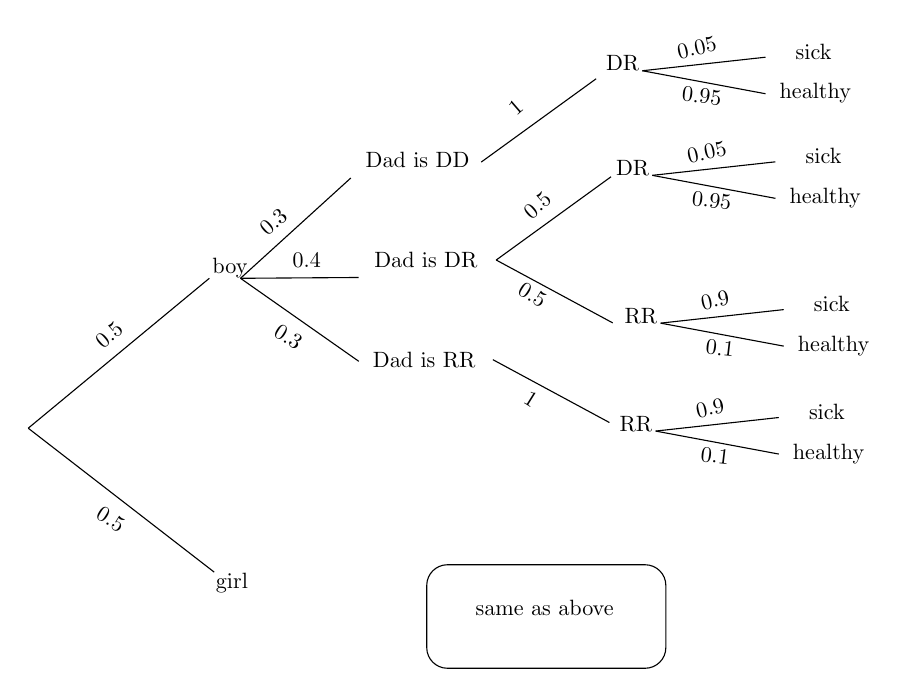
\begin{tikzpicture}[x=0.75pt,y=0.75pt,yscale=-1,xscale=1,scale=0.8,every node/.style={scale=0.8}]


	\draw    (70,322.1) -- (182,408.77) ;
	\draw    (70,322.1) -- (179.07,231.82) ;
	\draw    (264.27,171.42) -- (197.83,231.82) ;
	\draw    (197.83,231.82) -- (269.07,281.82) ;
	\draw    (197.83,231.82) -- (269,231.33) ;
	\draw    (412,111.67) -- (342.83,161.82) ;
	\draw    (420,318.67) -- (349.83,280.82) ;
	\draw    (422,258.67) -- (351.83,220.82) ;
	\draw    (421,170.67) -- (351.83,220.82) ;
	\draw    (514,120.67) -- (439.83,106.82) ;
	\draw    (514,98.67) -- (439.83,106.82) ;
	\draw    (520,183.67) -- (445.83,169.82) ;
	\draw    (520,161.67) -- (445.83,169.82) ;
	\draw    (525,272.67) -- (450.83,258.82) ;
	\draw    (525,250.67) -- (450.83,258.82) ;
	\draw    (522,337.67) -- (447.83,323.82) ;
	\draw    (522,315.67) -- (447.83,323.82) ;
	\draw   (310,416.8) .. controls (310,409.91) and (315.58,404.33) .. (322.47,404.33) -- (441.53,404.33) .. controls (448.42,404.33) and (454,409.91) .. (454,416.8) -- (454,454.2) .. controls (454,461.09) and (448.42,466.67) .. (441.53,466.67) -- (322.47,466.67) .. controls (315.58,466.67) and (310,461.09) .. (310,454.2) -- cycle ;
	
	\draw (191.47,225.3) node   [align=left] {boy};
	\draw (304.47,160.7) node   [align=left] {Dad is DD};
	\draw (192.67,415.5) node   [align=left] {girl};
	\draw (118.67,266) node  [rotate=-319.14] [align=left] {$\displaystyle 0.5$};	
	\draw (119.67,377) node  [rotate=-31.91] [align=left] {$\displaystyle 0.5$};
	\draw (226.67,267) node  [rotate=-31.91] [align=left] {0.3};
	\draw (217.67,198) node  [rotate=-319.14] [align=left] {$\displaystyle 0.3$};
	\draw (237.67,221) node  [rotate=-359.27] [align=left] {$\displaystyle 0.4$};
	\draw (309.47,220.7) node   [align=left] {Dad is DR};
	\draw (308.47,280.7) node   [align=left] {Dad is RR};
	\draw (363.67,129) node  [rotate=-319.14] [align=left] {$\displaystyle 1$};
	\draw (376.67,188) node  [rotate=-319.14] [align=left] {$\displaystyle 0.5$};
	\draw (373.67,242) node  [rotate=-31.91] [align=left] {0.5};
	\draw (372.67,305) node  [rotate=-31.91] [align=left] {1};
	\draw (472.67,93) node  [rotate=-347.27] [align=left] {$\displaystyle 0.05$};
	\draw (475.67,122) node  [rotate=-6.71] [align=left] {0.95};
	\draw (428,102.33) node   [align=left] {DR};
	\draw (543,95.33) node   [align=left] {sick};
	\draw (544,120.33) node   [align=left] {healthy};
	\draw (478.67,156) node  [rotate=-347.27] [align=left] {$\displaystyle 0.05$};
	\draw (481.67,185) node  [rotate=-6.71] [align=left] {0.95};
	\draw (434,165.33) node   [align=left] {DR};
	\draw (549,158.33) node   [align=left] {sick};
	\draw (550,183.33) node   [align=left] {healthy};
	\draw (483.67,245) node  [rotate=-347.27] [align=left] {$\displaystyle 0.9$};
	\draw (486.67,274) node  [rotate=-6.71] [align=left] {0.1};
	\draw (439,254.33) node   [align=left] {RR};
	\draw (554,247.33) node   [align=left] {sick};
	\draw (555,272.33) node   [align=left] {healthy};
	\draw (480.67,310) node  [rotate=-347.27] [align=left] {$\displaystyle 0.9$};
	\draw (483.67,339) node  [rotate=-6.71] [align=left] {0.1};
	\draw (436,319.33) node   [align=left] {RR};
	\draw (551,312.33) node   [align=left] {sick};
	\draw (552,337.33) node   [align=left] {healthy};
	\draw (381,430.33) node   [align=left] {same as above};
	
	
	\end{tikzpicture}
	\caption{Tree for problem 2.9}
	\label{fig:29}
\end{figure}

\clearpage

\end{document}
